\chapter{Description \& Methodology}

\section{FPGA}

The very heart of our computer is our custom made architecture implemented on our FPGA.
In this section we will first describe the overall architecture of our convolution engine before we will examine our implementation.

\subsection{Overall design}

Convolution is a very regular task where data flows only forward. This means that our processor can be simplified, removing the need for a central control module.
Instead each module simply operates under the assumption that all data inputs are correctly formatted and ordered and does its operations accordingly.

\section{Data in}

We used an EBI bus!

\section{Convolver}
In this section we will first focus on an idealized design to show the intent of our design without the added clutter introduced by implementation details before explaining our final design.
The two major parts of the convolution engine is the data feeder and the executing unit. By decoupling these we ensure a modular design allowing us to try a range of different approaches in our executing unit.
First we will give a brief description of the convolution process, this will also help us establish the necessary vocabulary. 
While our architecture aims to tackle many different kernel sizes we will use a 3 by 3 pixel convolution kernel and treat pixels as a single value rather than being composite of different colors like red green and blue.
In fig:Convolution the necessary operations for outputting a single pixel is shown. In each step each kernel is mapped according to some mapping function 
\begin{figure}[h!]
    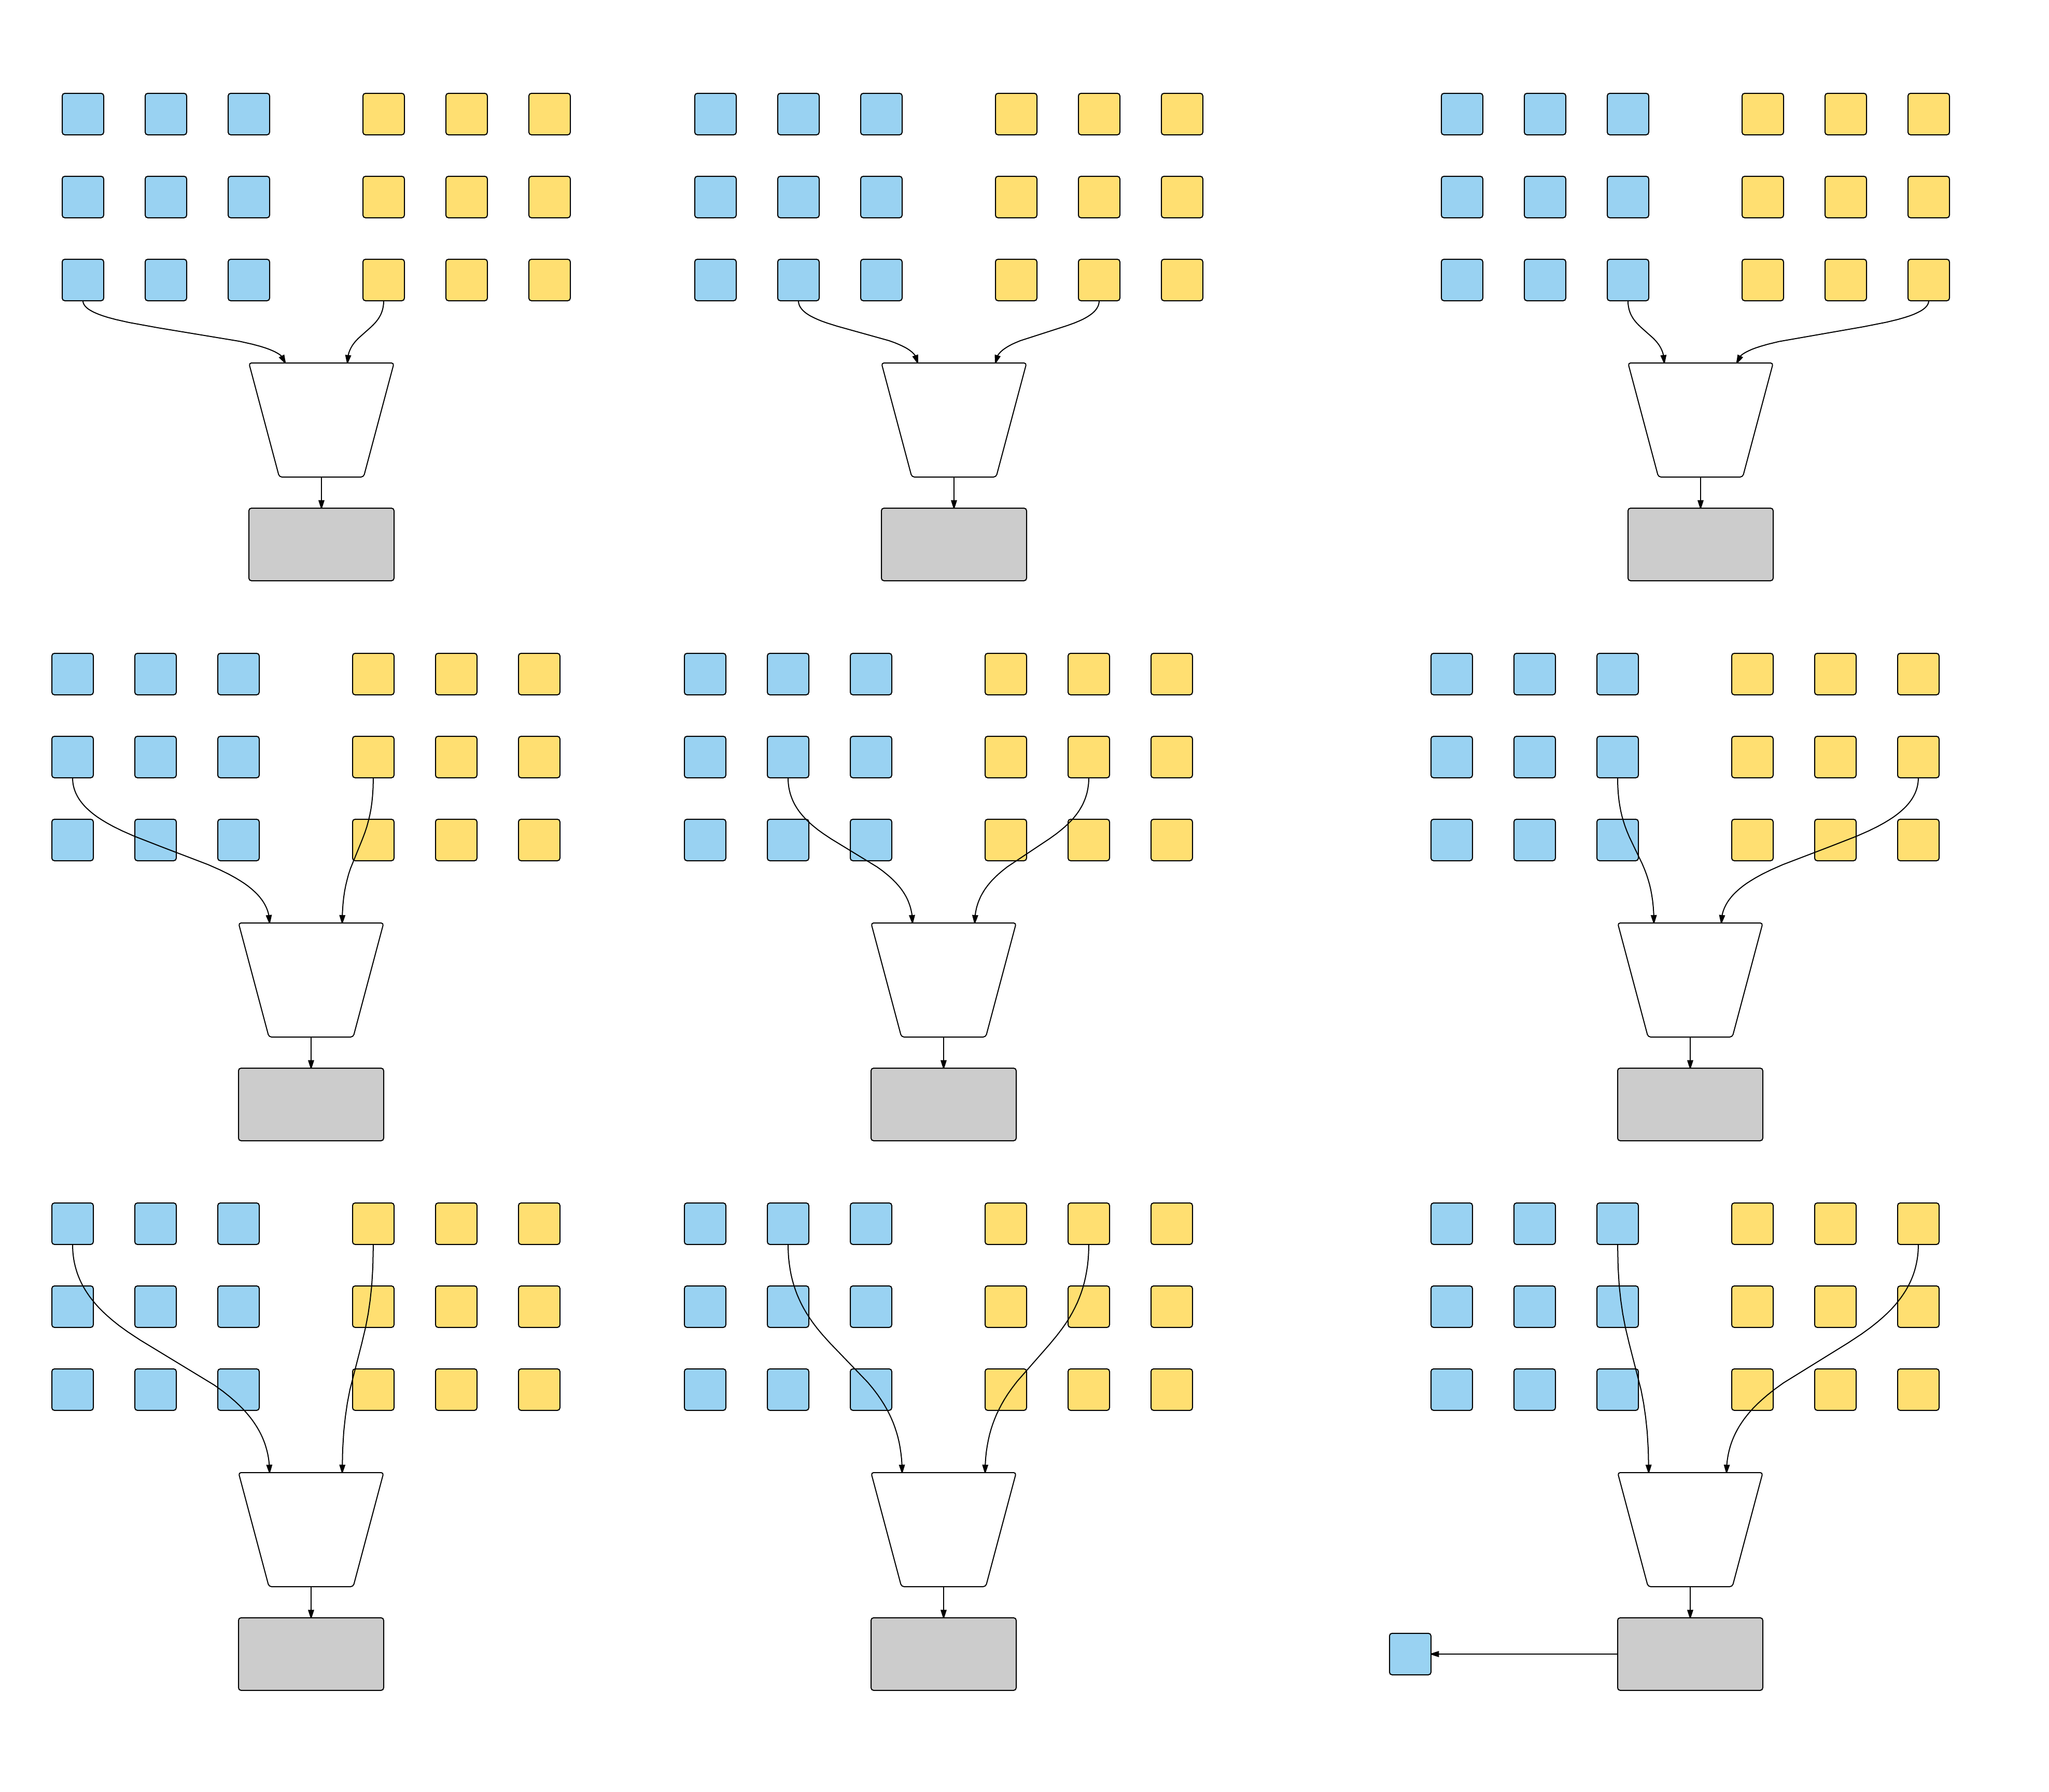
\includegraphics[width=\linewidth]{img/Convolution.png}
    \caption{The process of convoluting a single pixel}
    \label{fig:Convolution}
\end{figure}

On a larger scale, when we investigate the pixels of some image we see how each pixel is needed in several context. Fig:ContextsX shows three of the nine contexts in which the purple pixels is needed.
The concept of a context will be used to explain the data feeding operation, so readers should make themselves familiar with the terminology. 
In the figure the purple pixel is read in context of the convolution performed on the neighbourhood denoted by a gray background. 
When we write that some pixel A is read in the context of some other pixel B we mean that the pixel A is read in context of the convolution in which B is the center pixel. 
\begin{figure}[h!]
    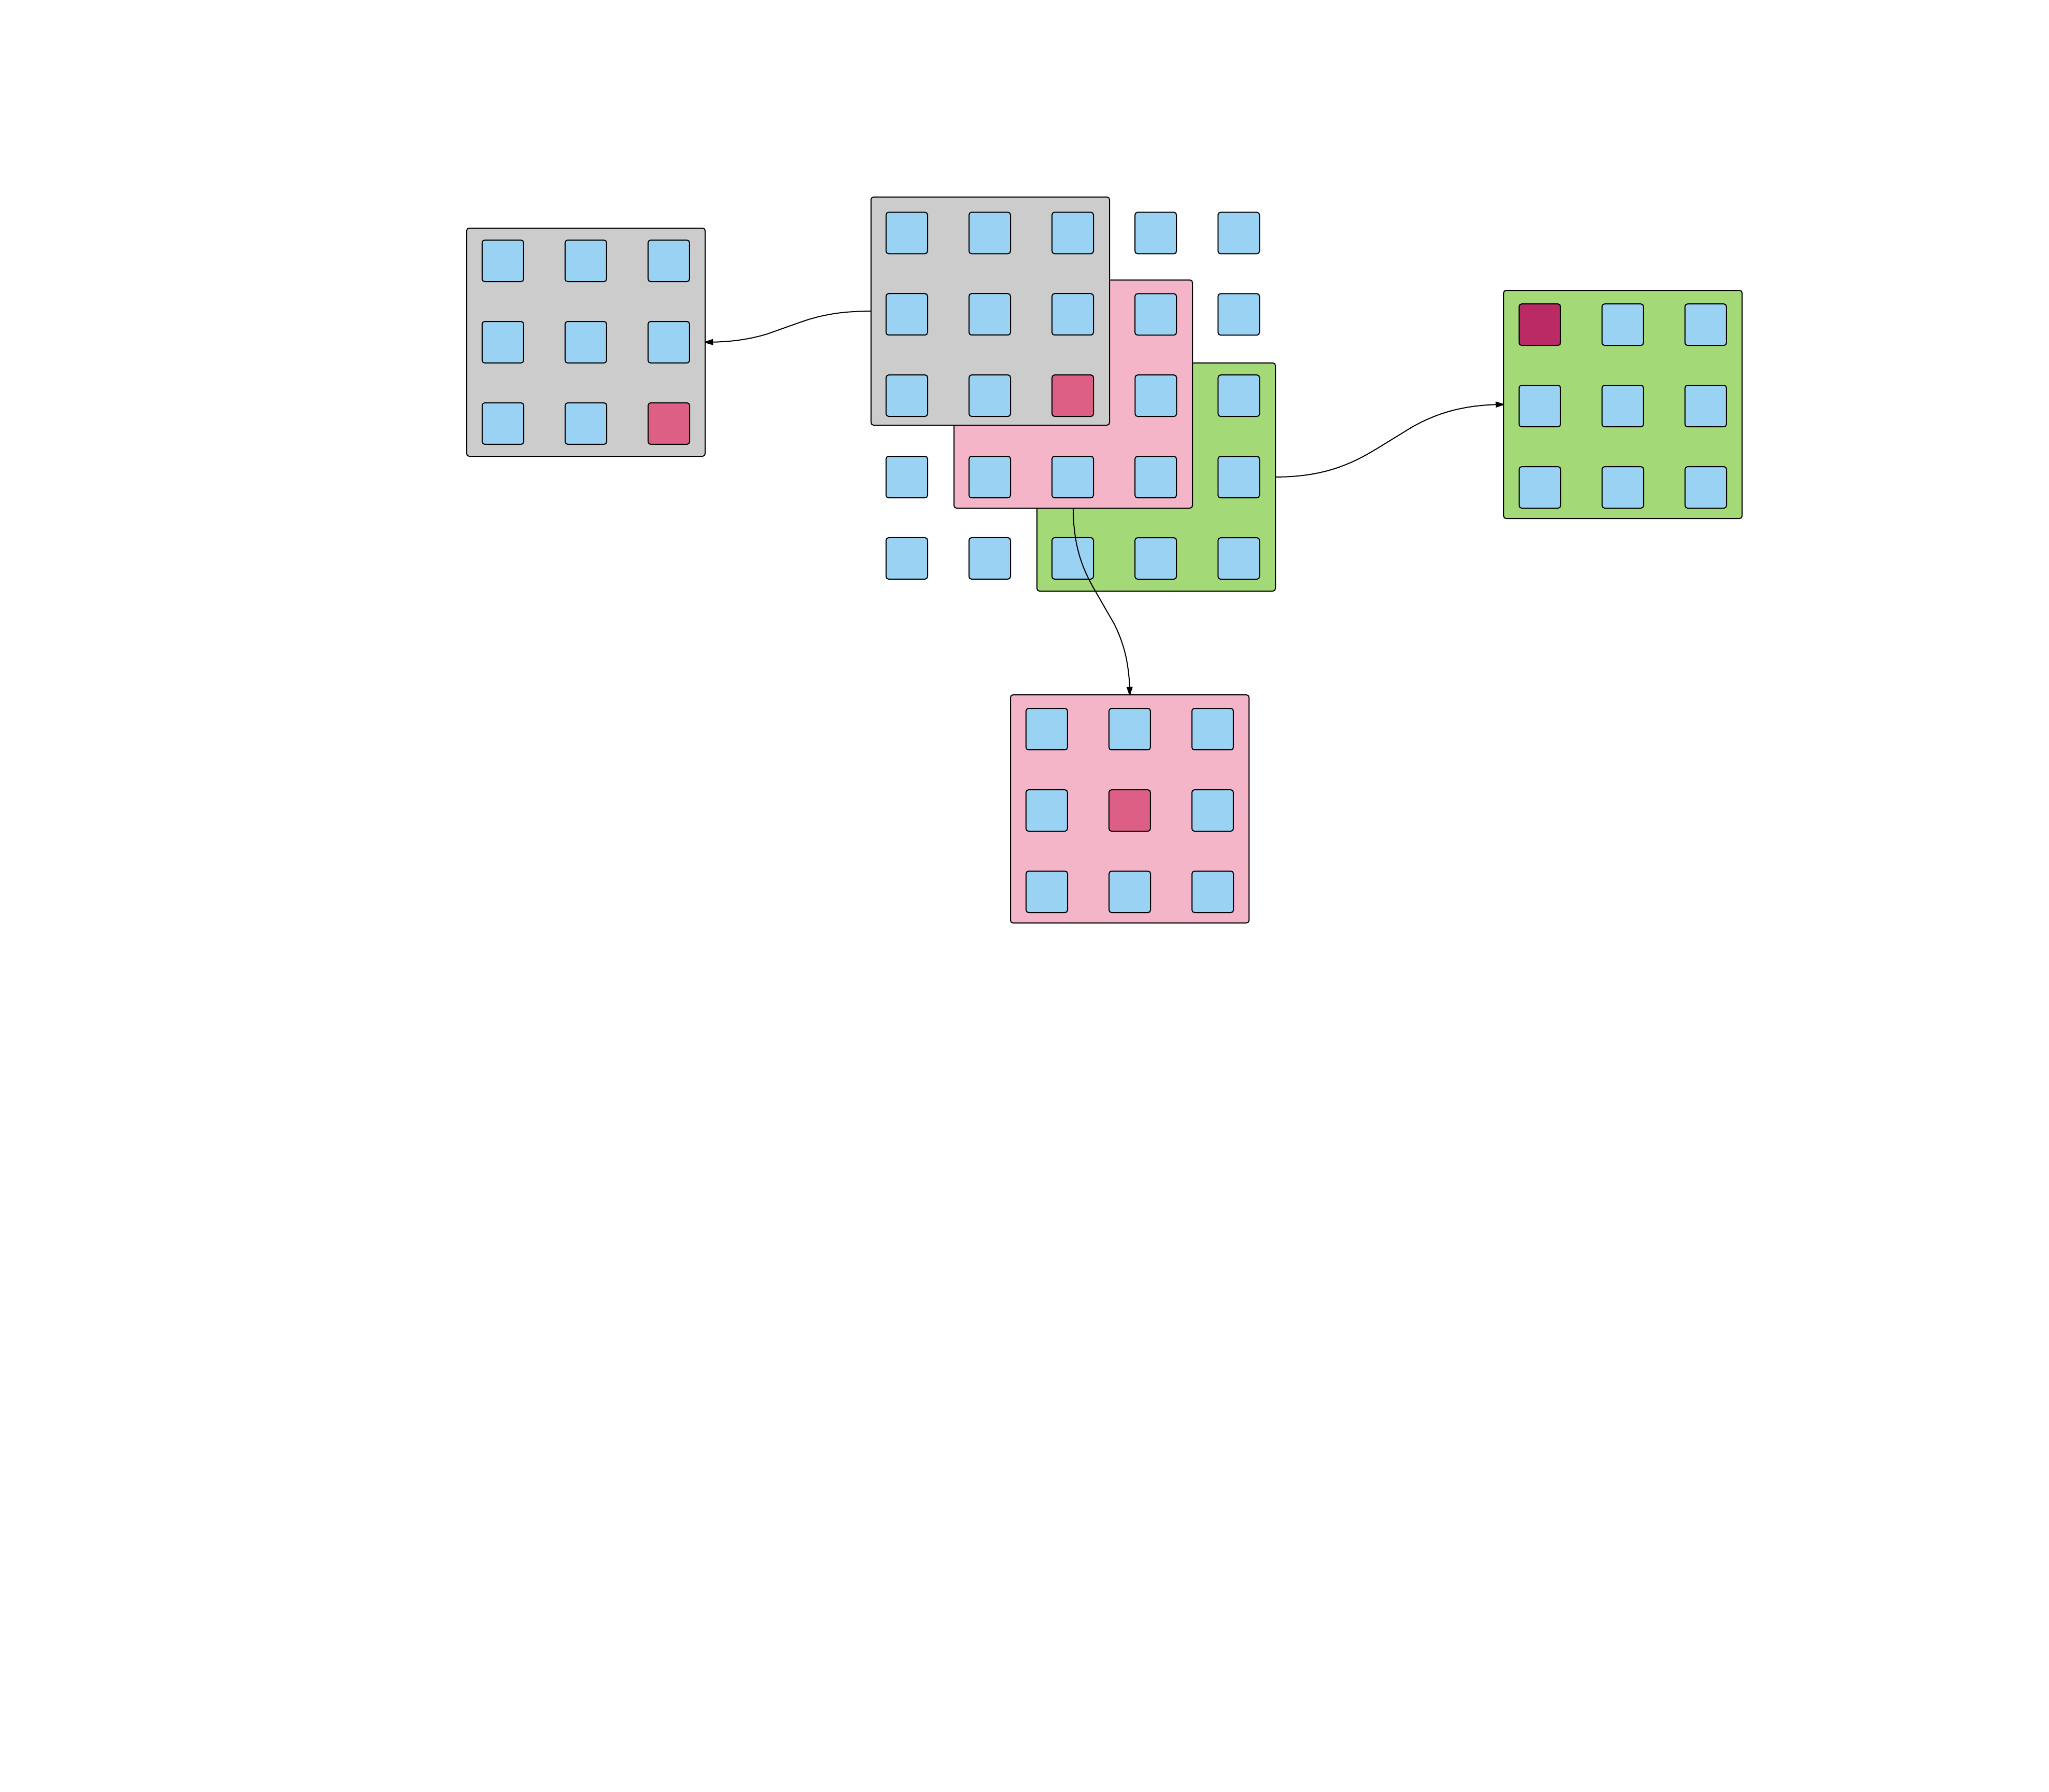
\includegraphics[width=\linewidth]{img/Contexts5.png}
    \caption{Three of the nine contexts a pixel is used}
    \label{fig:ConvolutionContexts}
\end{figure}


\subsection{Datafeeder}

\subsubsection{An ideal design}
The focal point of the convolver is the data delivery conveyor belt. This belt is a set of rows containing data, each row corresponding to a row in a convolution kernel.
In fig:Ideal we show an ideal version of the feeder consisting of three rows of pixels with an interconnect between each row.
Each cycle the convolver expects a datum from a FIFO queue which will be driven on the top interconnect, and each cycle exactly one register drives its value to the interconnect, and the register below it reads, transferring data laterally.
In our figure we show a feeder belt for a kernel of size 3*3 using nine columns. The green registers correspond to the register that is currently being extracted.
Each timestep the requested data is the register to the right of the previously requested register, wrapping around in a toroid fashion when the rightmost register was previously registered.
While the figure does not highlight it, in our ideal design we will assume that after a register has been read it responsible for reading from the interconnect as soon as the register above it drives the interconnect to ensure lateral data transfer.
In order to explain the purpose of our request pattern we will focus on the middle row, specifically the elements in this row that is surrounded by as many elements required by the convolution kernel.
In fig:Contexts these pixels are colored purple, and the surrounding pixels required to convolute the three first pixels are drawn with arrows pointing to the middle pixel.
Recall that when we refer to a pixel being read in context of another pixel, we mean that it is read in context of the convolution in which the other pixel is the middle pixel.
To motivate our reading pattern we will show three reads in the context of the three leftmost middle pixels in.
\begin{description}
  \item[$T_{1}$] \hfill \\
  The pixel read in the lowest row is read as southeast, south and southwest correspondingly by pixels 1, 2 and 3
  \item[$T_{2}$] \hfill \\
  The pixel read in the lowest row is read as southeast and south for middle pixels 2 and 3. middle pixel 1 is now done reading from the lower row and has started reading from the middle row.
  \item[$T_{3}$] \hfill \\
  Only the third middle pixel is still reading from the bottom row. Pixel one is now being read in context of itself, necessitating the split between contexts and actual pixels, while the second pixel is reading its left middle pixel
\end{description}
One observation we can make from this example is that once read a pixel will never be needed again in its current context. Thus after a register is read it will read the data from the row above it as soon as it is availible.
Until now we have simply talked a lot about context without discussing why it is important. After all, the data conveyor belt simply consists of three rows where each row iterates over its contents and outputs it.
The purpose of the design becomes clearer when we examine the three row outputs, and how the executing unit can obtain different parts of the conveyor belt by choosing which line to read from. 
Let us consider the timelapse in figure TODO. If an executing unit reads from row 3 at T1 to T3, then from row 2 at T4 to T6, and from rom 1 ad T7 to T0 it will have read all the pixels necessary for a convolution.
Had it started one timestep later it would have read all the necessary pixels to perform a convolution on the pixel right of the pixel from the previous read pattern and so on.
\begin{figure}[h!]
    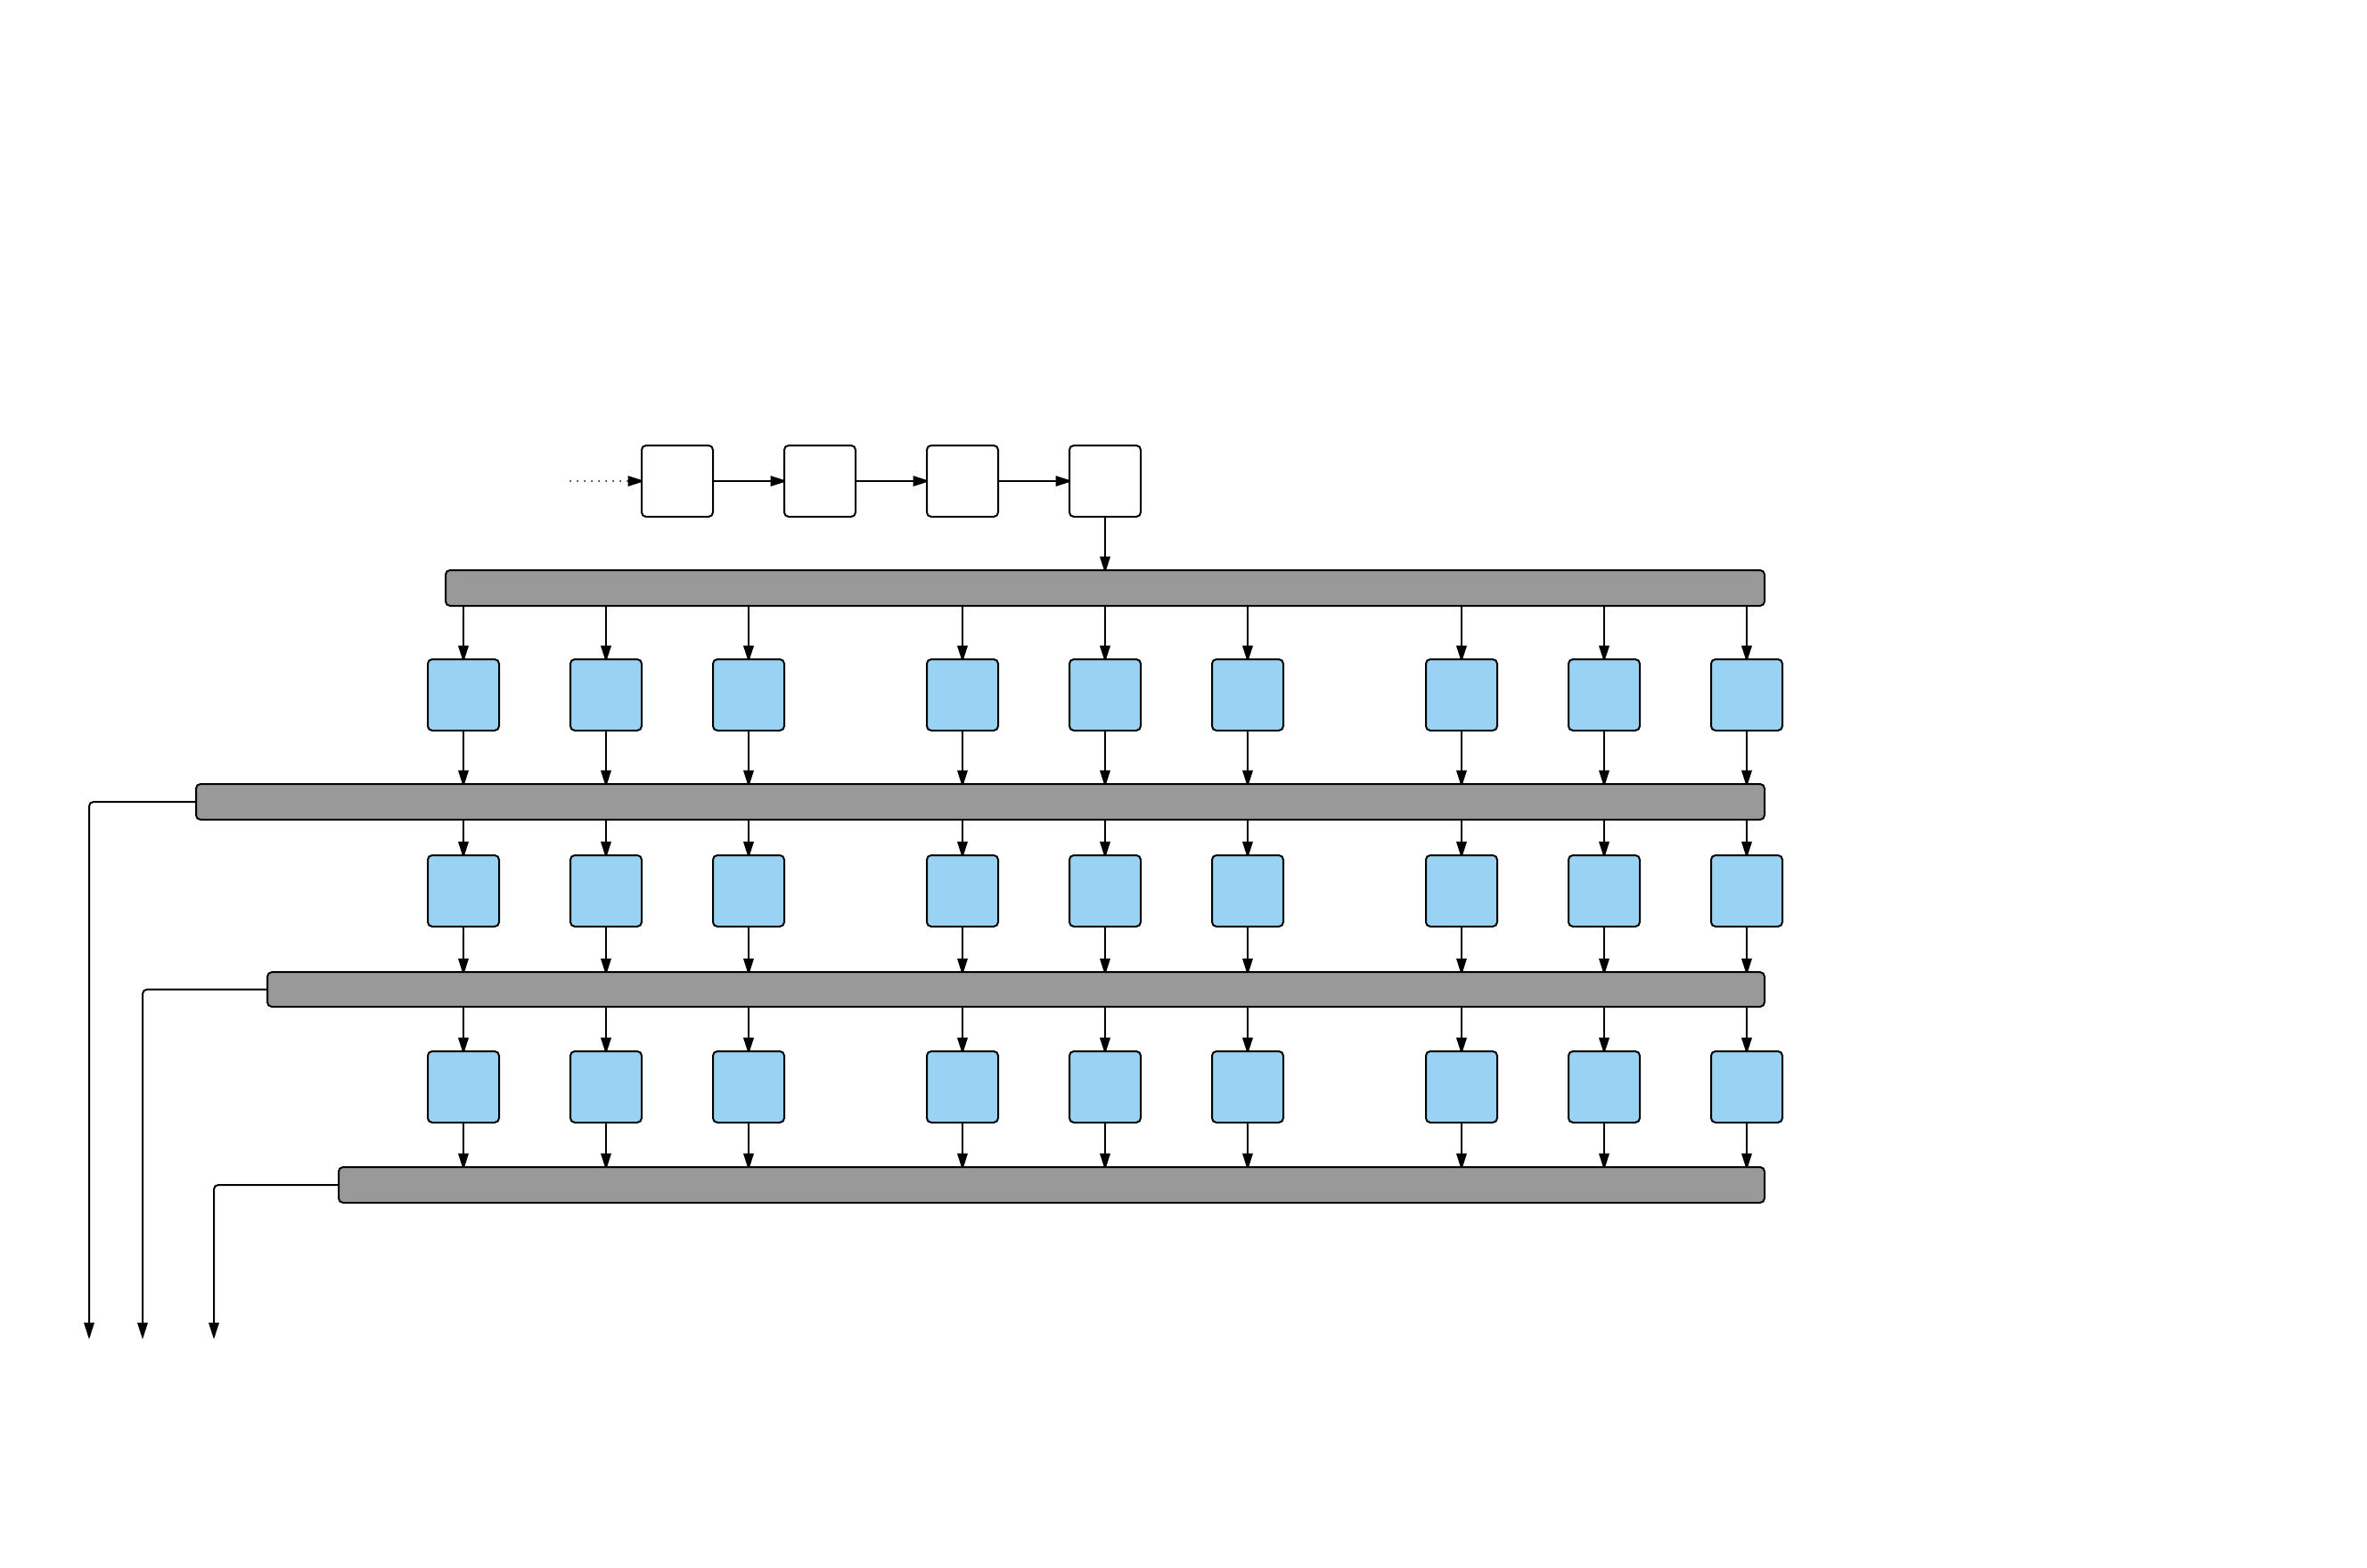
\includegraphics[width=\linewidth]{img/IdealFeeder.png}
    \caption{For each middle pixel, the contexts it applies to neighbouring pixels are denoted by arrows}
    \label{fig:Contexts}
\end{figure}

\begin{figure}[h!]
    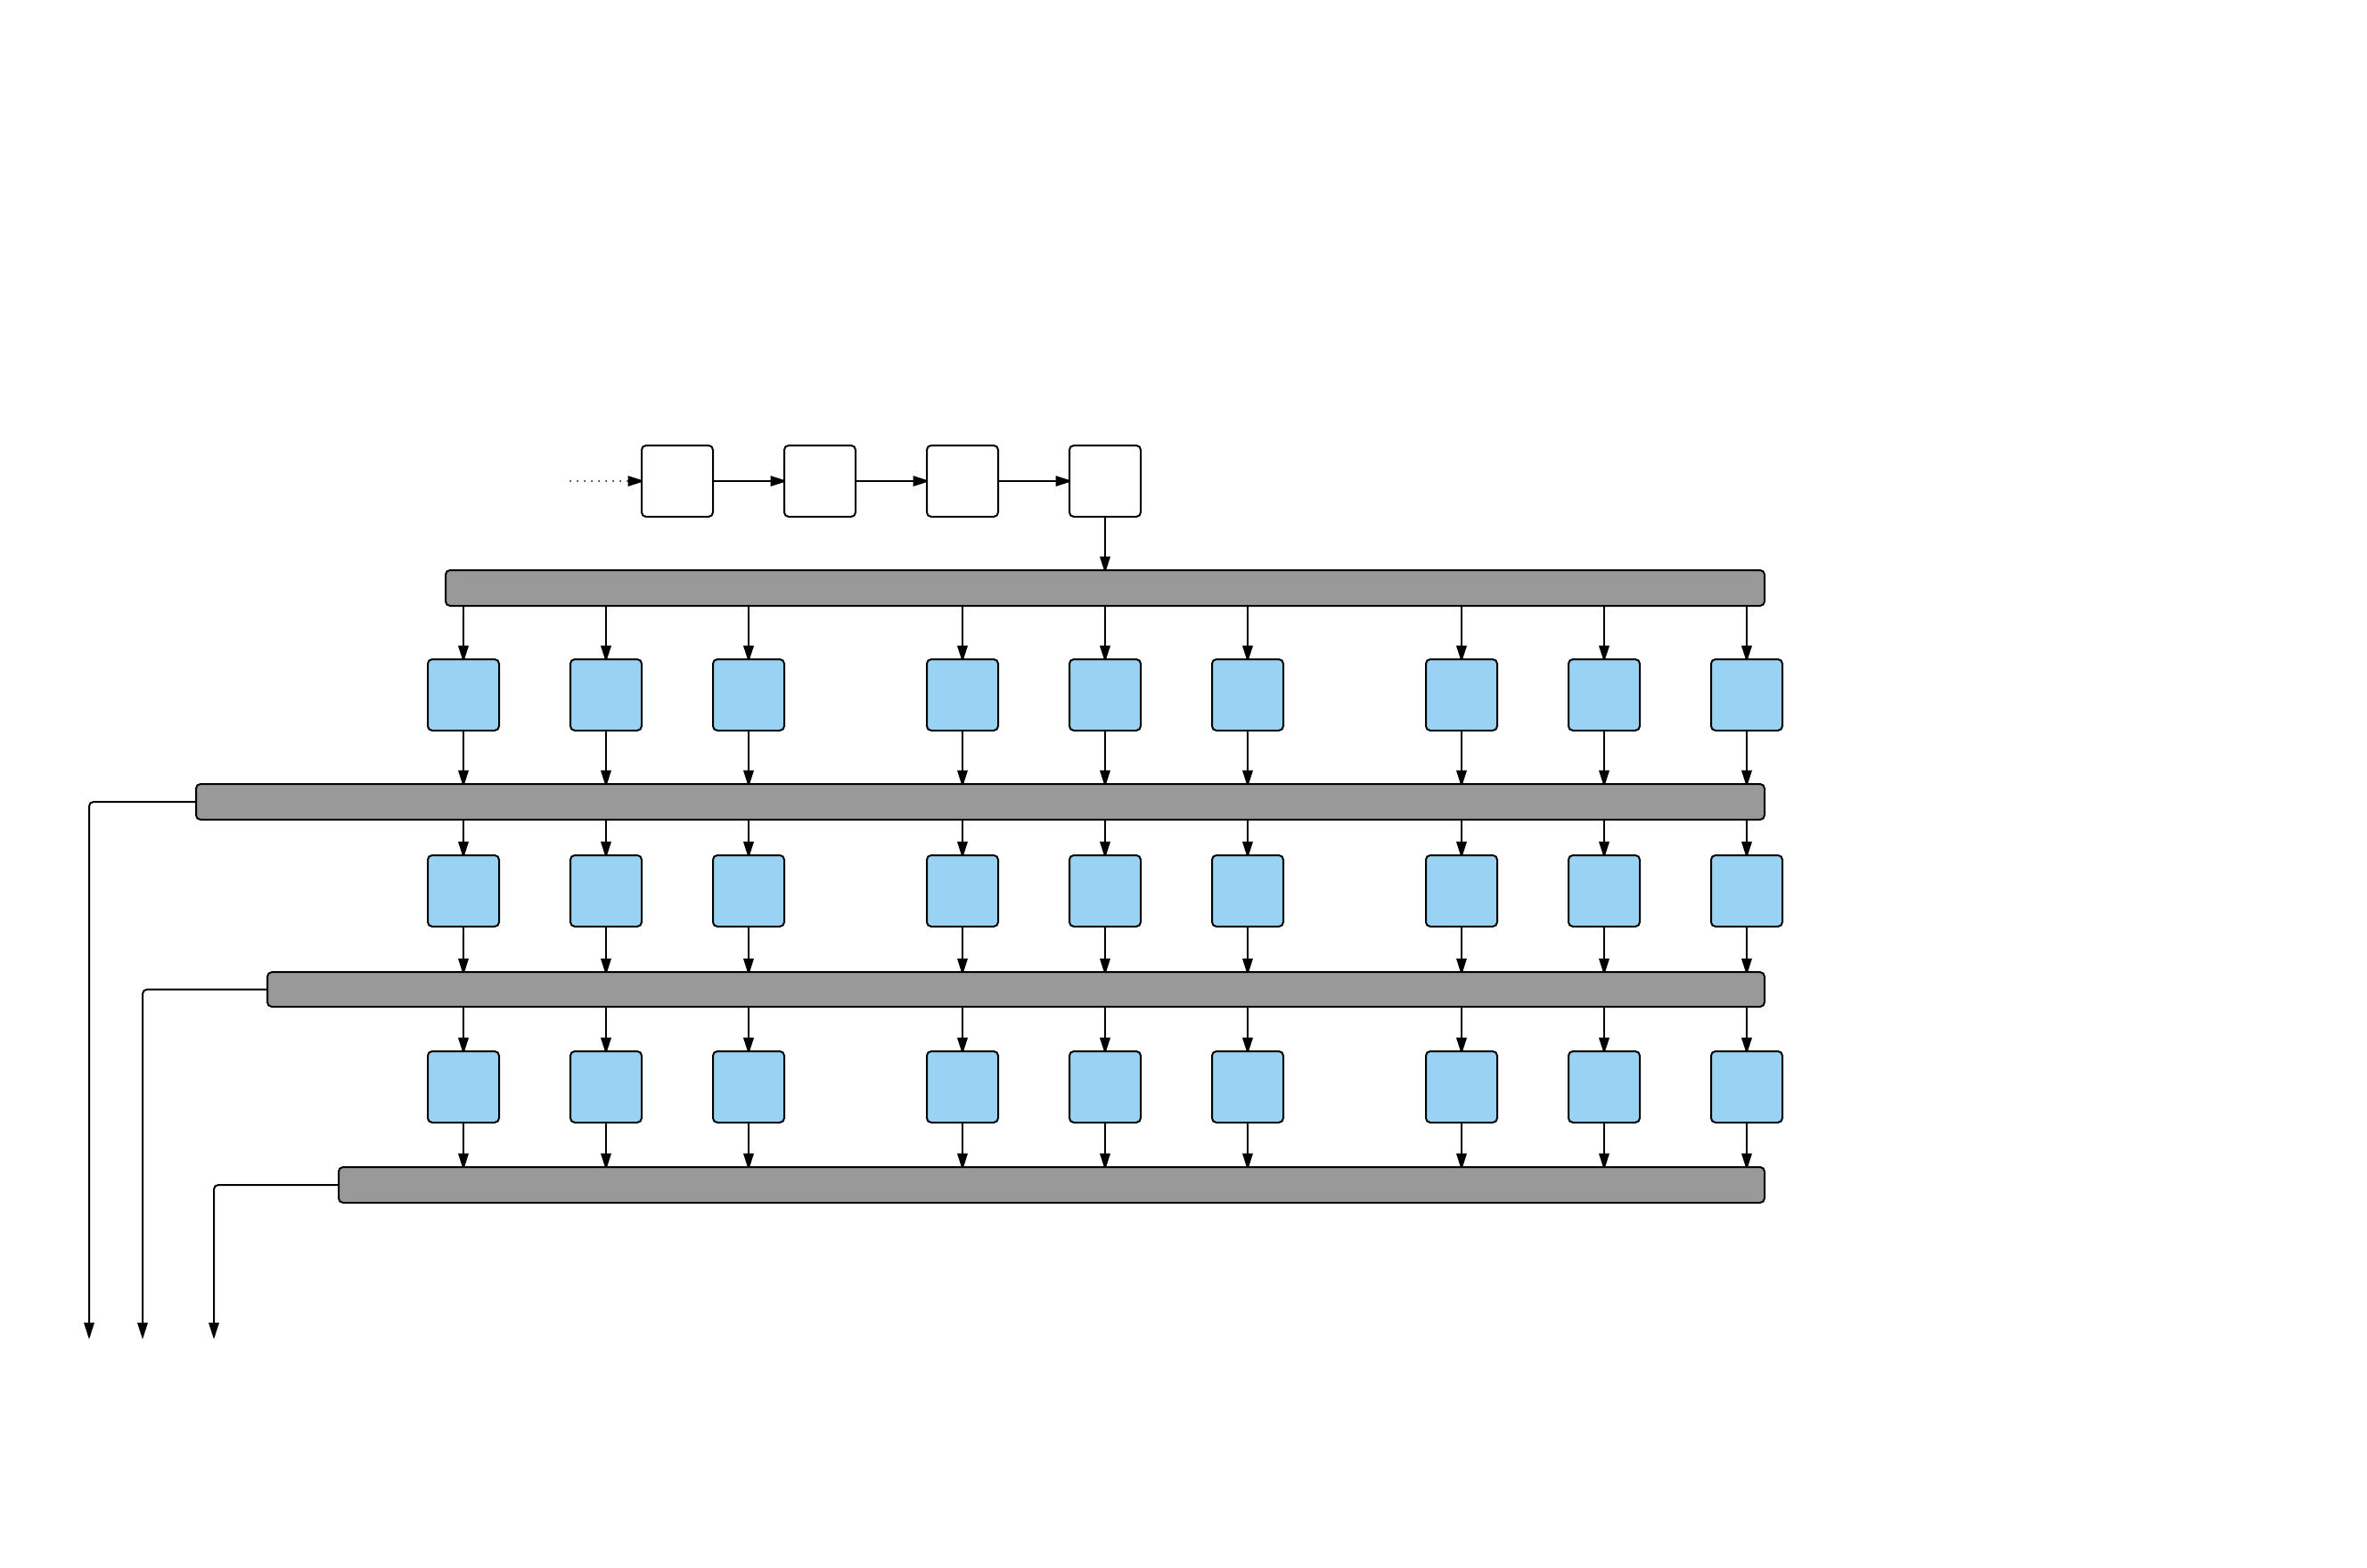
\includegraphics[width=\linewidth]{img/IdealFeeder.png}
    \caption{For each middle pixel, the contexts it applies to neighbouring pixels are denoted by arrows}
    \label{fig:Contexts}
\end{figure}
\subsubsection{An implementation}
In order to implement our ideal design we had to circumvent some limitations inherent to our FPGA. Primarily, FPGAs does not allow tri-state logic, forcing us to rely on a different approch than the interconnects in our ideal design.
Instead we used register balanced mux trees in order to extract data from rows as shown in fig: TODO.
In the 3x3 example each row has three multiplexers each, referred to as the primary multiplexers, and the pixel grid has its own multiplexers, one for each row, referred to as the secondary multiplexers.
Each primary multiplexer selects the register we want to read from that row if it is in range, else it selects an arbitrary register. The secondary multiplexer for the row selects the primary register whose output is currently valid.
We are now left with two instructions for each row. The registers need to enable reading, and the primary multiplexers needs to select the correct output. 
Rather than issuing these instructions from a central control module, we instead opted to daisy chain these instructions.
If we view the read signal for each register as a key, then each cycle the register which has the read key reads from the register above it and hands the key over to its right neighbour.
Similarily each primary multiplexer has three keyslots corresponding to the three registers above it. After daisychaining its key internally in its three slots it hands the key over to its right neighbour.
The control module is now simply responsible for issuing keys to the leftmost register and primary multiplexers, and then let the keys be shifted throughout the system.
Figuring out the timing for when keys are issued is not trivial, and we will not cover this here.
Suffice to say the timing can be crystallized into a simple state machine issuing keys at set intervals, and since the control state machine only interacts with the leftmost components it is easy to ensure correctness.

